% =============================================================================
% Appendix B: User Manual
% =============================================================================
\chapter{User Manual}
\label{app:user-manual}

\small
This appendix provides step-by-step instructions for installing, configuring, and running the \textsc{SciFig-Eval} system. The system comprises three main components: a Python-based evaluation pipeline that generates and scores figure descriptions, an adversarial experiment suite that stress-tests model behaviour, and a React dashboard for interactive exploration of results.

\section{System Requirements}

Table~\ref{tab:sys-req} lists the software and credentials required. At least one API provider is needed; the system supports mixing providers (e.g., Azure for GPT-5.2 and OpenRouter for open-weight models) within a single evaluation run.

\begin{table}[H]
\centering
\scriptsize
\caption{System requirements.}\label{tab:sys-req}
\begin{tabular}{@{}l l p{6cm}@{}}
\toprule
\textbf{Component} & \textbf{Version} & \textbf{Details} \\
\midrule
Python       & 3.11+  & Tested on 3.12 \\
Node.js      & 20+    & For the dashboard (npm 10+) \\
API keys     & ---    & OpenRouter, Azure OpenAI, or GCP Vertex AI \\
Python pkgs  & ---    & \texttt{openai}, \texttt{google-genai}, \texttt{python-dotenv}, \texttt{numpy}, \texttt{matplotlib}, \texttt{scipy} \\
Disk space   & 2\,GB  & Full dataset and outputs \\
\bottomrule
\end{tabular}
\end{table}

\section{Installation and Setup}

The repository is self-contained: all dataset figures, groundtruth annotations, and experiment benchmarks are included. After cloning, only Python dependencies and API credentials are needed.

\begin{enumerate}[leftmargin=*]
\item \textbf{Clone and install:}
\begin{codebox}[title={\scriptsize Shell}]
{\scriptsize git clone <repo-url> SciFig-Evaluation && cd SciFig-Evaluation
python3 -m venv .venv && source .venv/bin/activate
pip install openai google-genai python-dotenv numpy matplotlib scipy seaborn}
\end{codebox}

\item \textbf{Configure \texttt{.env}:} Create a \texttt{.env} file in the project root with your API credentials. The system loads these automatically via \texttt{python-dotenv}.
\begin{codebox}[title={\scriptsize Environment variables}]
{\scriptsize OPENROUTER_API_KEY=sk-or-...
AZURE_OPENAI_ENDPOINT=https://your-resource.openai.azure.com/
AZURE_OPENAI_API_KEY=...
GCP_PROJECT=your-gcp-project-id}
\end{codebox}
\end{enumerate}

\section{Evaluation Pipeline}

The evaluation pipeline operates in three sequential stages, illustrated in Figure~\ref{fig:pipeline-flow}. Each stage reads from the previous stage's output directory and writes structured JSON files. The \texttt{--workers} flag controls concurrent API calls; all scripts skip figures that already have output files, making re-runs safe and incremental.

\begin{figure}[H]
  \centering
  
\includegraphics[width=\textwidth]{figures/pipeline_flow.pdf}
  \caption{Evaluation pipeline data flow. Stage~1 generates descriptions for all 1,005 figures across 13 models. Stage~2 scores each description using two LLM judges under three configurations. Stage~3 computes aggregate results and plots.}
  \label{fig:pipeline-flow}
\end{figure}

\noindent\textbf{Stage 1: Generate model descriptions.} Each model processes every figure in the dataset, receiving the image and a language-specific prompt. The runner automatically selects the correct prompt template based on figure type and language. Output is one JSON file per figure containing the model's description.
\begin{codebox}[title={\scriptsize Generation}]
{\scriptsize python3 scripts/llm_generation/run.py gpt-5.2 --workers 4
python3 scripts/llm_generation/run.py gemini-3.1-pro --subfolder english_only
# Output: output/generation/<model>/<subfolder>/<fig_key>.json}
\end{codebox}

\noindent\textbf{Stage 2: Run MQM evaluation.} Two LLM judges (GPT-4o and Mistral Large~3) independently score each model's description under three configurations. Judge~A sees only the image; Judge~B sees only the groundtruth; Judge~C sees both. Each judge returns categorised errors with severity levels.
\begin{codebox}[title={\scriptsize MQM Evaluation}]
{\scriptsize python3 scripts/evaluation/evaluate_reference_free.py gpt-5.2 --judge azure/gpt-4o
python3 scripts/evaluation/evaluate_reference_only.py gpt-5.2 --judge azure/gpt-4o
python3 scripts/evaluation/evaluate_reference_with_image.py gpt-5.2 --judge azure/gpt-4o
# Output: output/evaluation/<judge_type>/<judge>/<model>/<subfolder>/<fig>.json}
\end{codebox}

\noindent\textbf{Stage 3: Compute results.} Aggregation scripts read all evaluation JSONs, compute bootstrap confidence intervals, pairwise significance tests, and per-language breakdowns, and generate the tables and plots reported in the thesis.
\begin{codebox}[title={\scriptsize Results computation}]
{\scriptsize python3 scripts/evaluation-results/rq1/compute_leaderboard.py
python3 scripts/evaluation-results/rq2/compute_degradation.py
python3 scripts/evaluation-results/rq3/compute_capability.py
python3 scripts/evaluation-results/rq4/compute_ari.py}
\end{codebox}

\section{Adversarial Experiments}

The adversarial suite evaluates model behaviour under stress using a curated 45-figure subset (9 per language, balanced across chart types). Each experiment type targets a specific behavioural dimension: image transforms test robustness (RQ2), caption bias and prompt reversal test resistance (RQ4), capability questions test comprehension (RQ3), and admittance/inductance probes test honesty and reasoning (RQ4). Table~\ref{tab:adv-commands} lists the runner commands.

\begin{table}[H]
\centering
\scriptsize
\caption{Adversarial experiment commands. All operate on the 45-figure subset.}\label{tab:adv-commands}
\begin{tabular}{@{}l p{8cm}@{}}
\toprule
\textbf{Experiment} & \textbf{Command} \\
\midrule
Image transforms  & \texttt{python3 scripts/experiments/run\_transforms.py gpt-5.2 --workers 4} \\
Caption bias      & \texttt{python3 scripts/experiments/run\_caption\_bias.py gpt-5.2 --condition modified\_caption} \\
Prompt reversal   & \texttt{python3 scripts/experiments/run\_prompt\_reverse.py gpt-5.2 --workers 4} \\
Capability Qs     & \texttt{python3 scripts/experiments/run\_questions.py gpt-5.2 --prompt 1 --workers 4} \\
Inductance        & \texttt{python3 scripts/experiments/run\_inductance.py --model gemini-3.1-pro} \\
Active admittance & \texttt{python3 scripts/experiments/run\_active\_admittance.py --model gpt-5.2 --workers 4} \\
\bottomrule
\end{tabular}
\end{table}

\section{Dashboard}

The interactive dashboard provides a browser-based interface for exploring the full dataset, reviewing individual judge evaluations with colour-coded error annotations, and comparing model performance across languages and conditions. It is built with React~19, Vite~7, Tailwind CSS~4, and Recharts~3.

\begin{codebox}[title={\scriptsize Launch dashboard}]
{\scriptsize cd dashboard/ && npm install && npm run dev   # http://localhost:5173}
\end{codebox}

\noindent The dashboard is organised into three tabs: \textbf{Dataset} (browse figures, annotations, adversarial probes, and inferable elements), \textbf{Evaluation} (inspect MQM error annotations, compare transforms, review adversarial probe responses), and \textbf{Results} (leaderboard tables, cross-model analytics, and per-judge breakdowns). In production, figures and data are served from Azure Blob Storage; in development, they are loaded from the local \texttt{public/} directory.

\section{Reproducing Thesis Results}

Each table and figure in the thesis is generated by a single Python script. Table~\ref{tab:result-scripts} maps thesis artefacts to their computation scripts. All scripts read from \texttt{output/} and write results to \texttt{output/evaluation-results/}. Plots are saved as both PDF (for LaTeX) and PNG (for the dashboard).

\begin{table}[H]
\centering
\scriptsize
\caption{Mapping of thesis artefacts to computation scripts (paths relative to \texttt{scripts/}).}
\label{tab:result-scripts}
\begin{tabular}{@{}l l@{}}
\toprule
\textbf{Thesis artefact} & \textbf{Script} \\
\midrule
Table 6.1 (Leaderboard)       & \texttt{evaluation-results/rq1/compute\_leaderboard.py} \\
Table 6.1b (Error analysis)    & \texttt{evaluation-results/rq1/compute\_error\_analysis.py} \\
Figure 6.1a (Heatmap)          & \texttt{evaluation-results/rq1/plot\_heatmap.py} \\
Figure 6.1b (Error stacked)    & \texttt{evaluation-results/rq1/plot\_error\_stacked.py} \\
Table 6.2 (Degradation)        & \texttt{evaluation-results/rq2/compute\_degradation.py} \\
Figure 6.4 (Slope chart)       & \texttt{evaluation-results/rq2/plot\_degradation\_slope.py} \\
Table 6.3 (Capability)         & \texttt{evaluation-results/rq3/compute\_capability.py} \\
Table 6.4 (A-R-I scores)       & \texttt{evaluation-results/rq4/compute\_ari.py} \\
Figure 7.1 (Rank flow)         & \texttt{evaluation-results/discussion/plot\_rank\_flow.py} \\
Figure 7.2 (A-R-I scatter)     & \texttt{evaluation-results/discussion/plot\_ari\_scatter.py} \\
\bottomrule
\end{tabular}
\end{table}

% =============================================================================
% Appendix C: Maintenance Manual
% =============================================================================
\chapter{Maintenance Manual}
\label{app:maintenance-manual}

\small
This appendix documents the internal architecture of \textsc{SciFig-Eval} to support ongoing development, extension to new models and languages, and long-term maintenance. It assumes familiarity with Python, REST APIs, and the evaluation concepts described in the main text.

\section{Repository Structure}

The repository follows a separation between source data (\texttt{Dataset/}), experiment definitions (\texttt{adversarial\_experiments/}), executable code (\texttt{scripts/}), and generated outputs (\texttt{output/}). This separation ensures that re-running any stage overwrites only its own output directory without affecting upstream data. Table~\ref{tab:repo-structure} summarises the key directories.

\begin{table}[H]
\centering
\scriptsize
\caption{Repository structure. Only key directories shown.}\label{tab:repo-structure}
\begin{tabular}{@{}l p{8.5cm}@{}}
\toprule
\textbf{Path} & \textbf{Purpose} \\
\midrule
\texttt{Dataset/figures/}           & PNG images in 5 language subfolders (english\_only, german\_only, bulgarian\_only, chinese\_only, multi\_language) \\
\texttt{Dataset/groundtruth/}       & JSON annotations with paper metadata, captions, and human descriptions (same subfolders) \\
\texttt{adversarial\_experiments/}   & 45-figure adversarial subset: probe benchmarks, transform definitions, source PDFs \\
\texttt{atomic\_mqm/atoms/}          & 120 atomic MQM decomposition JSONs mapping figures to verifiable fact checklists \\
\texttt{scripts/llm\_generation/}    & Model abstractions (\texttt{models.py}), prompt templates, generation runners \\
\texttt{scripts/evaluation/}         & MQM judge pipeline (\texttt{mqm\_evaluator.py}), backend routing, export utilities \\
\texttt{scripts/experiments/}        & Adversarial experiment runners and evaluators (one per experiment type) \\
\texttt{scripts/evaluation-results/} & Result computation and plotting scripts organised by research question \\
\texttt{output/}                     & All generated artefacts: descriptions, evaluations, experiment results, tables, plots \\
\texttt{dashboard/}                  & React + Vite + Tailwind interactive dashboard (src/pages/, public/data/) \\
\texttt{HumanEval/}                  & Label Studio exports and processed human evaluation data \\
\texttt{thesis/}                     & LaTeX thesis source, figures, and bibliography \\
\bottomrule
\end{tabular}
\end{table}

\section{Code Architecture}

The codebase is built around two core abstractions: a model layer that normalises access to heterogeneous VLM APIs, and a judge pipeline that produces comparable MQM scores regardless of which judge configuration is used.

\subsection{Model Abstraction Layer}

All thirteen VLMs are accessed through the \texttt{FigureAnnotator} abstract base class defined in \texttt{scripts/llm\_generation/models.py}. Figure~\ref{fig:class-hierarchy} shows the class hierarchy. Each concrete annotator handles API-specific details (authentication, request format, token encoding) behind a uniform interface. The factory function \texttt{get\_annotator(name)} resolves a model name string to the correct annotator class by consulting three registries: \texttt{AZURE\_MODELS} (for Azure-deployed models like GPT-5.2), \texttt{OPENROUTER\_MODELS} (for open-weight models routed through OpenRouter), and \texttt{CUSTOM\_TOKEN\_MODELS} (for models requiring non-default token limits).

\begin{figure}[H]
  \centering
  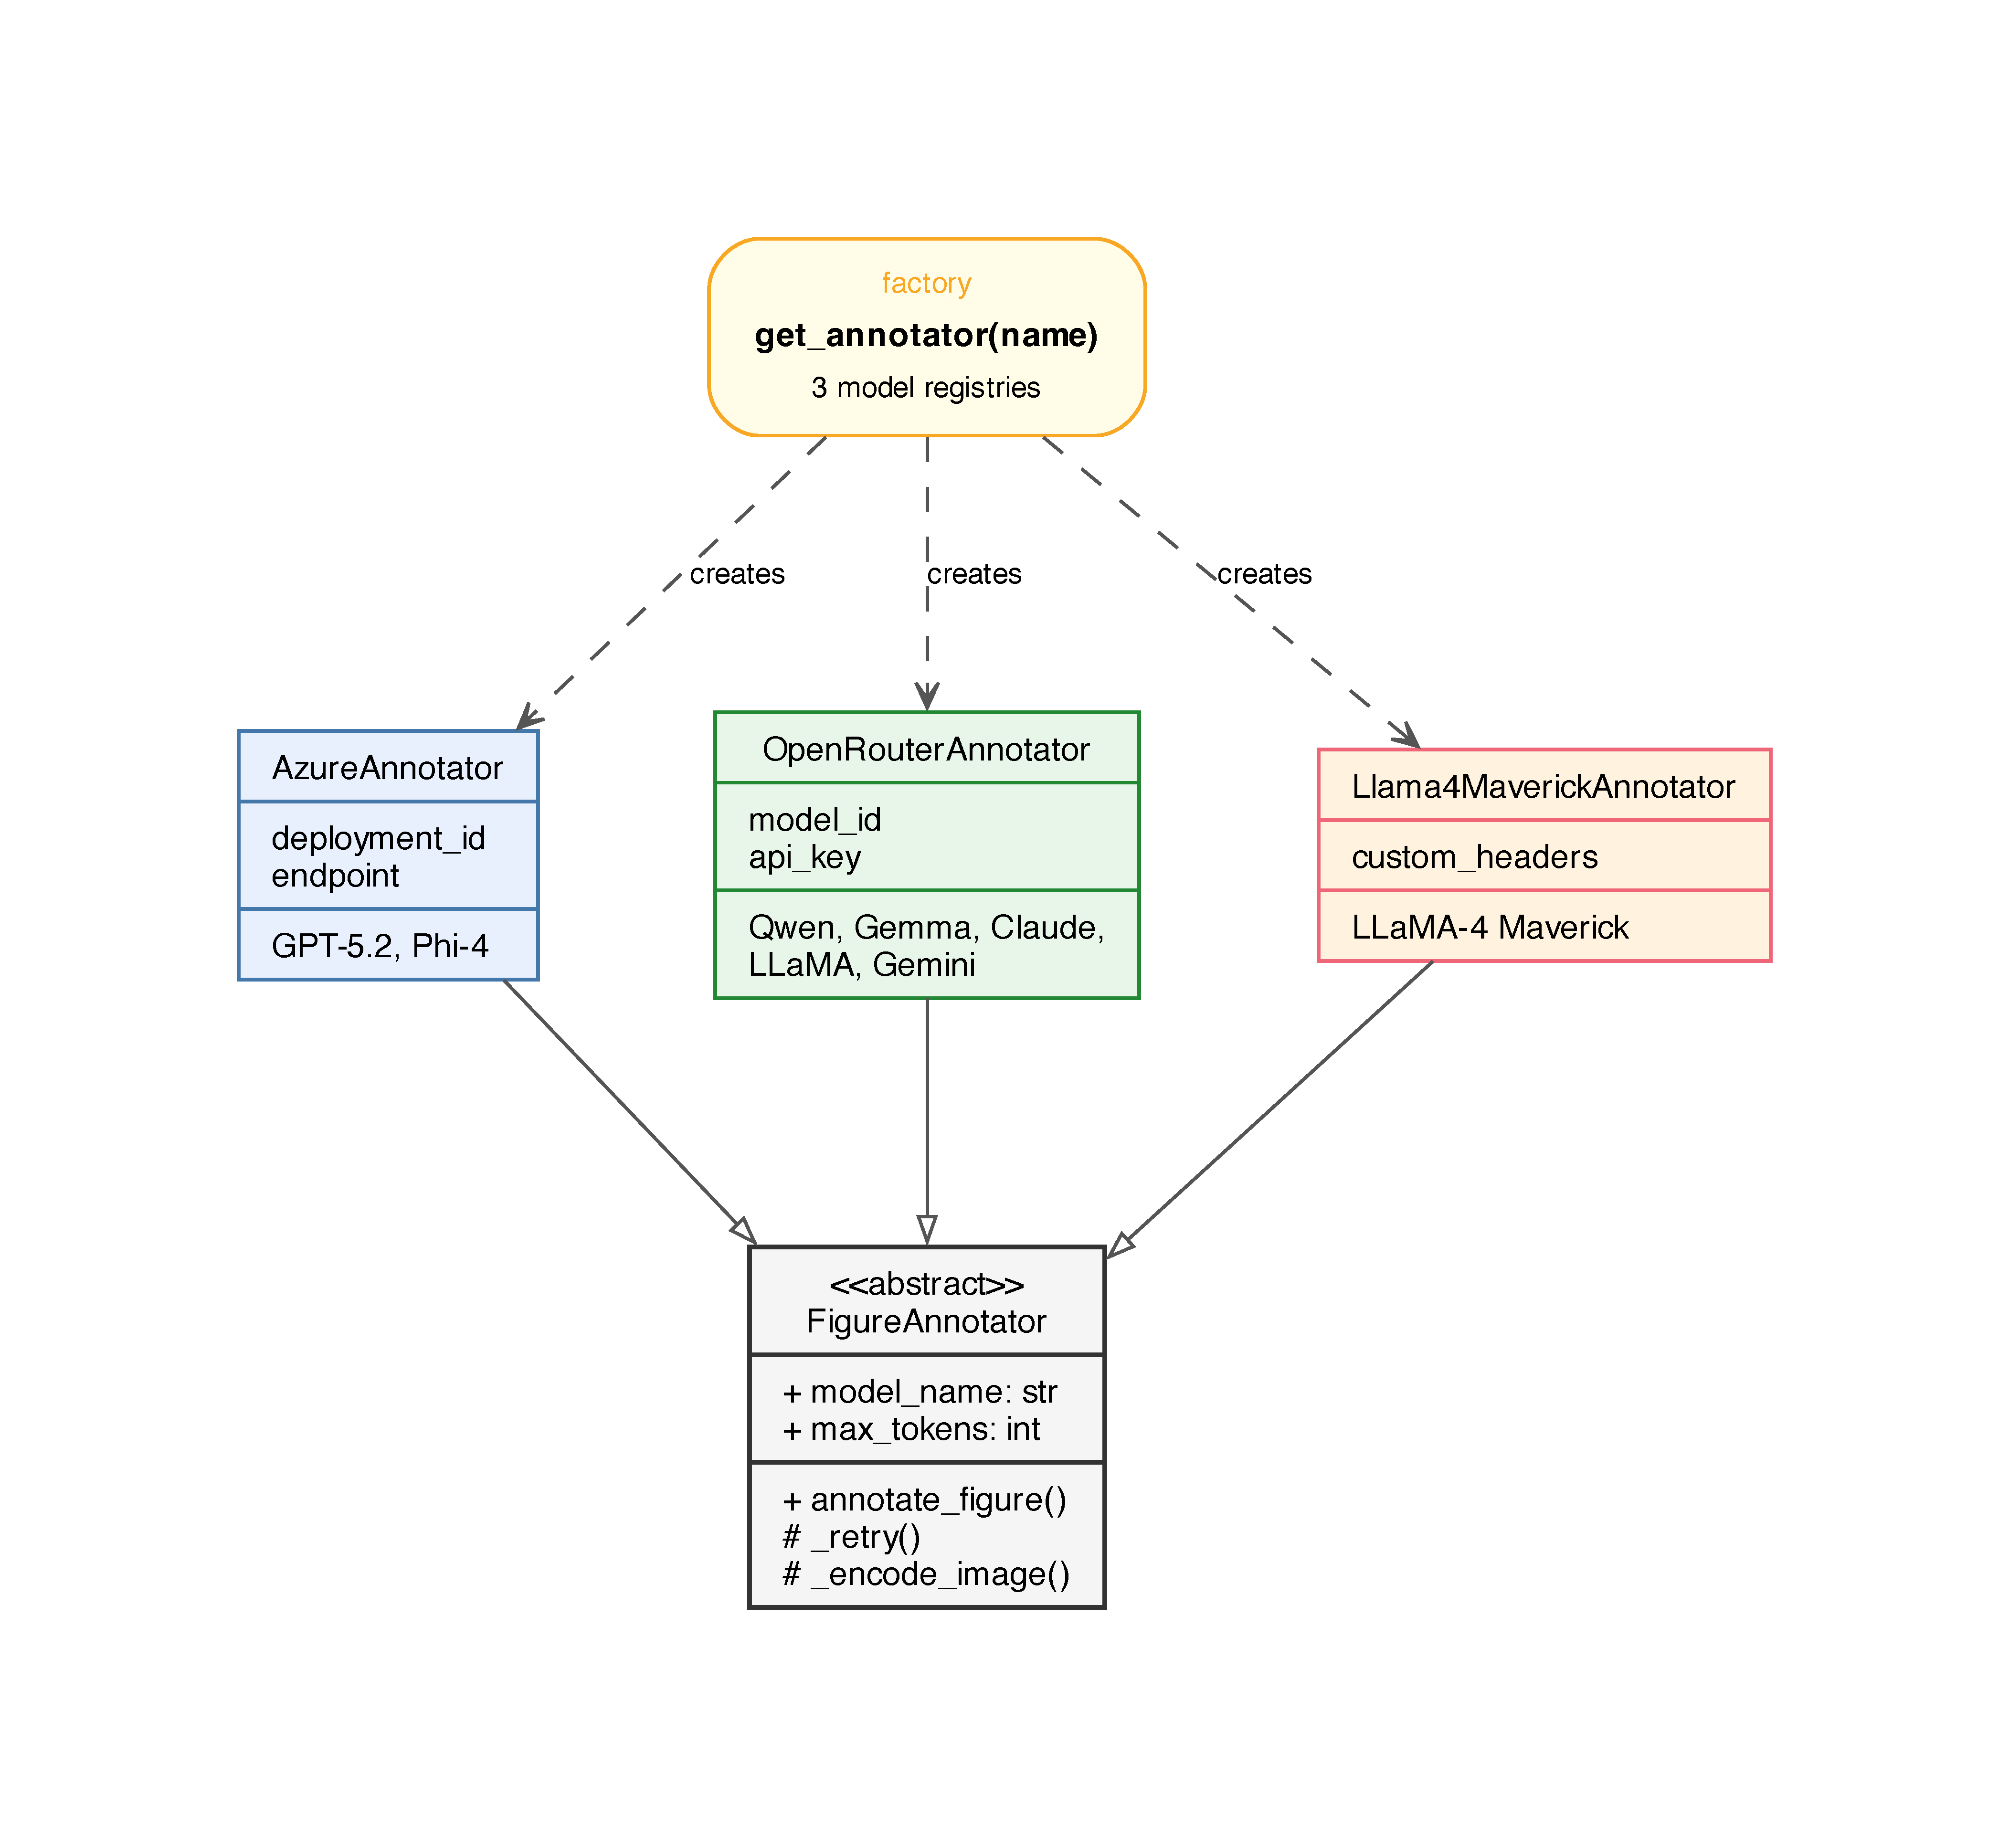
\includegraphics[width=0.75\textwidth]{figures/class_hierarchy.pdf}
  \caption{UML class diagram: \texttt{FigureAnnotator} hierarchy and factory pattern. Each annotator implements \texttt{annotate\_figure()}, which encodes the image as Base64, constructs the API request, and returns the generated description. A shared \texttt{\_retry()} wrapper handles transient failures with exponential backoff (maximum three attempts).}
  \label{fig:class-hierarchy}
\end{figure}

\subsection{Judge Pipeline}

The MQM evaluation system in \texttt{scripts/evaluation/mqm\_evaluator.py} implements three judge configurations, each providing a different trade-off between evaluation rigour and input requirements. Judge routing is configured in \texttt{judge\_backends.json}, which maps model prefixes to API backends: \texttt{azure/*} routes to Azure OpenAI, \texttt{gemini-*} to Vertex AI, and all others to OpenRouter.

\begin{table}[H]
\centering
\scriptsize
\caption{Judge configurations and their inputs.}
\begin{tabular}{@{}l l l@{}}
\toprule
\textbf{Judge} & \textbf{Inputs} & \textbf{Truth source} \\
\midrule
A (Reference-free)       & Image + prompt + caption + output & Image \\
B (Reference-only)       & Groundtruth + output              & Reference \\
C (Reference-with-image) & Image + groundtruth + output      & Image (primary) \\
\bottomrule
\end{tabular}
\end{table}

\noindent Each judge returns a structured JSON with categorised errors. Errors are scored using the MQM weight table: Accuracy Major/Minor (5.0/2.0), Completeness Major/Minor (3.5/1.5), Clarity Major/Minor (2.0/1.0). The final MQM score is normalised to 0--100 using the atom count as denominator.

\section{Adding New Models}

The model abstraction layer is designed for easy extension. To add a new VLM:

\begin{enumerate}[leftmargin=*]
\item \textbf{Register the model} in the appropriate dictionary in \texttt{scripts/llm\_generation/models.py}. The key is the model name string used in CLI commands; the value is the provider-specific identifier.
\begin{codebox}[title={\scriptsize models.py}]
{\scriptsize OPENROUTER_MODELS["new-model"] = "provider/model-id"
# or: AZURE_MODELS["new-model"] = "deployment-name"
# or: CUSTOM_TOKEN_MODELS["new-model"] = ("provider/id", 16000)}
\end{codebox}

\item \textbf{For a new API backend} (i.e., not Azure, OpenRouter, or Vertex AI), subclass \texttt{FigureAnnotator}, implement \texttt{annotate\_figure()} and the \texttt{model\_name} property, and register the class in \texttt{MODEL\_REGISTRY}.

\item \textbf{Run the full pipeline} for the new model. The scripts will create output directories automatically.
\begin{codebox}[title={\scriptsize Run new model}]
{\scriptsize python3 scripts/llm_generation/run.py new-model --workers 4
python3 scripts/evaluation/evaluate_reference_free.py new-model --judge azure/gpt-4o}
\end{codebox}
\end{enumerate}

\section{Adding New Languages}

The system's multilingual support is based on language-specific subfolders and prompt templates. To add a new language:

\begin{enumerate}[leftmargin=*]
\item Place figure images in \texttt{Dataset/figures/<lang>\_only/}
\item Create groundtruth JSON annotations in \texttt{Dataset/groundtruth/<lang>\_only/} following the existing schema (\texttt{task\_id}, \texttt{arxiv\_id}, \texttt{paper\_title}, \texttt{paper\_language}, \texttt{figure\_type}, \texttt{caption}, \texttt{annotations})
\item Write generation prompt templates in \texttt{scripts/llm\_generation/prompts/cross\_language/} for each figure type (bar chart, line plot, pie chart, default)
\item Create atomic MQM decomposition files in \texttt{atomic\_mqm/atoms/} if using the atomic evaluator
\item Add the new subfolder name to the \texttt{SUBFOLDERS} list in \texttt{run.py} and all evaluator scripts
\item Update \texttt{SUBFOLDER\_TO\_LANGUAGE} and \texttt{LANG\_MAP} dictionaries in the results computation scripts
\end{enumerate}

\section{Configuration Reference}

Table~\ref{tab:config-ref} lists all environment variables and key configuration files. All API calls use \texttt{temperature=0} to ensure deterministic, reproducible outputs. The retry mechanism in both generation and evaluation uses exponential backoff with a maximum of three attempts.

\begin{table}[H]
\centering
\scriptsize
\caption{Environment variables and key configuration files.}\label{tab:config-ref}
\begin{tabular}{@{}l l p{5cm}@{}}
\toprule
\textbf{Variable / File} & \textbf{Used by} & \textbf{Description} \\
\midrule
\texttt{OPENROUTER\_API\_KEY}       & OpenRouter models & API key for all OpenRouter-hosted models \\
\texttt{AZURE\_OPENAI\_ENDPOINT}    & Azure models      & Azure OpenAI resource URL \\
\texttt{AZURE\_OPENAI\_API\_KEY}    & Azure models      & Azure OpenAI API key \\
\texttt{GCP\_PROJECT}               & Vertex AI         & Google Cloud project ID for Gemini \\
\midrule
\texttt{.env}                        & All scripts       & Central environment variable store \\
\texttt{judge\_backends.json}        & Evaluation        & Maps judge model prefixes to API backends \\
\texttt{models.py}                   & Generation        & Model registry, annotator classes, factory \\
\texttt{samples.json}                & Experiments       & 45-figure adversarial sample manifest \\
\bottomrule
\end{tabular}
\end{table}

% =============================================================================
% Appendix D: Ethics Statement
% =============================================================================
\chapter{Ethics Statement}
\label{app:ethics-detail}

\small
This appendix provides full details on the ethical considerations governing human annotation and data collection in this project.

\paragraph{Data sources.}
All 1,005 scientific figures are drawn from publicly available papers on arXiv, Wirtschaftsdienst, CCL/ACL Anthology, and ISA/UNWE Sofia. No copyrighted material was reproduced beyond fair-use figure excerpts for research evaluation purposes. No personally identifiable information appears in the dataset.

\paragraph{Annotator recruitment and consent.}
Eight annotators were recruited to produce the 1,411 ground-truth annotations across four languages. All annotators participated voluntarily and were briefed on the project objectives, annotation guidelines, and expected time commitment prior to commencing work. Annotators were informed that their contributions would be used for academic research and were free to withdraw at any time without consequence.

\paragraph{Data anonymisation.}
No personally identifiable information about annotators is stored in the dataset. Annotations are identified only by anonymous annotator IDs (numeric identifiers with no mapping to real identities in the published dataset). The annotation task involved describing publicly available scientific figures and posed no foreseeable risk to participants.

\paragraph{Ethical compliance.}
The study was conducted in accordance with the University of Aberdeen's ethical guidelines for research involving human participants. The annotation task falls within the category of minimal-risk research: participants performed a professional task (describing scientific figures) using publicly available materials, with no deception, no sensitive personal data collected, and no foreseeable harm.

\paragraph{Bias and equity.}
VLM performance varies substantially across languages, with Bulgarian figures receiving the lowest-quality descriptions, which has direct implications for equitable access to scientific content. We report these disparities transparently to inform deployment decisions.

\paragraph{Evaluation and deployment.}
The thirteen VLMs were accessed through commercial APIs (Azure OpenAI, OpenRouter, Google Vertex AI) under standard terms of service. No model weights were modified, and all evaluations used deterministic settings (\texttt{temperature=0}) to ensure reproducibility.
The dual-judge evaluation inherits biases from GPT-4o and Mistral Large~3, including the severity split documented in Chapter~\ref{ch:discussion}. We mitigate this through judge averaging and human validation, but acknowledge that the evaluation framework reflects the perspectives of two specific commercial models.
Even the best-performing model produces ${\sim}2.7$ incorrect numerical values per figure; we caution against deploying VLM-generated descriptions as authoritative without human verification, particularly in contexts where numerical precision is critical.

% =============================================================================
% Appendix F: Comparison to Existing Benchmarks
% =============================================================================
\chapter{Comparison to Existing Benchmarks}
\label{app:benchmark-comparison}

\small
Table~\ref{tab:benchmark-comparison} positions \textsc{SciFig-Eval} against seven established chart and figure understanding benchmarks.
Existing benchmarks predominantly evaluate extraction accuracy through closed-form question answering (short answer, multiple choice, or binary), using a single accuracy metric on English-only datasets.
\textsc{SciFig-Eval} differs in three respects: it evaluates open-ended description generation using a multidimensional MQM quality framework, it covers four typologically diverse languages sourced from native-language venues, and it introduces adversarial probes and behavioural metrics (Admittance, Resistance, Inductance) that no existing benchmark measures.

The RQ3 capability questions are the closest equivalent to existing QA benchmarks, and the findings align: counting and comparison are the hardest question types across both \textsc{SciFig-Eval} and ChartQA/CharXiv, while extraction of individual values is comparatively easier.
However, the key contribution of \textsc{SciFig-Eval} is what lies beyond accuracy: the A-R-I behavioural profiles reveal failure modes (silent fabrication, resistance gaps, sycophantic agreement) that QA benchmarks structurally cannot detect because they test only correctness, not honesty or robustness.
A model scoring 90\% on ChartQA may still fabricate under blur and accept false premises --- behaviours that only surface under adversarial evaluation.

\begin{table}[H]
\centering
\scriptsize
\caption{Comparison of \textsc{SciFig-Eval} to existing chart/figure understanding benchmarks.}\label{tab:benchmark-comparison}
\setlength{\tabcolsep}{2pt}
\begin{tabular}{@{}l l r l l l l@{}}
\toprule
\textbf{Benchmark} & \textbf{Task} & \textbf{Scale} & \textbf{Langs} & \textbf{Metric} & \textbf{Adv.} & \textbf{Behav.} \\
\midrule
ChartQA        & Short-answer QA   & 32.7K QA   & EN    & Relaxed Acc. & No  & No \\
CharXiv        & Short-answer QA   & 2.3K QA    & EN    & Accuracy     & No  & No \\
MMMU           & Multiple-choice   & 11.5K QA   & EN    & Accuracy     & No  & No \\
PlotQA         & Short-answer QA   & 28.9M QA   & EN    & Accuracy     & No  & No \\
SciFIBench     & Fig--caption match & 2K QA     & EN    & Accuracy     & No  & No \\
PolyChartQA    & Short-answer QA   & 26.2K QA   & 10    & Accuracy     & No  & No \\
ChartMuseum    & Short-answer QA   & 1.2K QA    & EN    & Accuracy     & No  & No \\
\midrule
\textbf{SciFig-Eval} & \textbf{Open description} & \textbf{1K figs} & \textbf{4} & \textbf{MQM} & \textbf{Yes} & \textbf{A-R-I} \\
\bottomrule
\end{tabular}
\end{table}

\noindent PolyChartQA is the only other multilingual benchmark but covers a different language set (no Bulgarian or German), uses generated rather than real scientific figures, and evaluates QA accuracy only.
ChartMuseum and CharXiv are the most challenging existing benchmarks (GPT-4o achieves 47\% on CharXiv reasoning, 63\% on ChartMuseum) but remain within the closed-form QA paradigm.
\textsc{SciFig-Eval} is complementary to these benchmarks: it addresses the behavioural dimensions they do not cover, while they provide extraction accuracy baselines that \textsc{SciFig-Eval} does not replicate.

\section{Dual-Judge Design}

The evaluation uses two LLM judges (GPT-4o and Mistral Large~3) rather than a single judge or a larger panel. This design reflects three considerations.
First, cross-provider diversity: GPT-4o (OpenAI via Azure) and Mistral Large~3 (Mistral AI via Azure) represent different model families with different training data and biases, reducing the risk that scoring patterns reflect a single provider's idiosyncrasies.
Second, the severity split between judges (GPT-4o assigns 78\% Major vs Mistral's 47\% on identical errors) is itself a finding: it reveals that absolute MQM scores are judge-dependent while rankings are robust ($\rho_{\text{sys}}\geq.95$). A single judge would mask this disagreement.
Third, practical constraints: each additional judge doubles evaluation cost. At approximately 9,360 judge calls for the 120-figure sample alone, adding a third judge would have required reducing the model or figure count.
Open-weight judges were considered but not used because, at the time of evaluation, no open-weight model matched GPT-4o or Mistral Large~3 on structured JSON output reliability, which is essential for the atomic MQM scoring pipeline.

\section{End-to-End Behavioural Probing}

The adversarial probes in \textsc{SciFig-Eval} test end-to-end model behaviour rather than isolating individual pipeline stages (visual encoder, alignment layer, language decoder).
This is a deliberate design choice: deployment contexts care about whether a model fabricates, not whether the fabrication originates in the encoder or the decoder.
A model that correctly encodes a blurred region but whose decoder fabricates a confident answer is functionally equivalent, from a user's perspective, to a model whose encoder fails to detect the blur entirely.
The A-R-I framework therefore measures behavioural outcomes (admittance, resistance, inductance) rather than internal mechanisms.
Mechanistic attribution of these behaviours to specific pipeline stages is identified as future work (\S\ref{sec:future-work}), requiring techniques such as attention visualisation and activation probing that fall outside the scope of this evaluation-focused thesis.

\section{Data Contamination}

The English (arXiv) and Chinese (CCL/ACL Anthology) figures in the corpus are drawn from venues whose papers are almost certainly present in the pre-training data of closed-weight models such as GPT-5.2, Gemini 3.1 Pro, and Claude Opus 4.6. This means that English and Chinese results may partly reflect memorisation of previously seen figures rather than genuine visual comprehension. By contrast, the Bulgarian (ISA/UNWE Sofia) and German (Wirtschaftsdienst) figures are drawn from smaller, domain-specific venues that are less likely to appear in large-scale web crawls, making these subsets more genuinely out-of-distribution.
This asymmetry could plausibly account for a portion of the cross-lingual performance gap observed in Table~6.1, where English and Chinese scores tend to be higher than Bulgarian. The controlled cross-lingual experiment (\S\ref{sec:rq1-ablations}) partially mitigates this concern by using parallel figures across all four languages, but it cannot fully disentangle the contribution of memorisation from that of genuine multilingual capability. Future work could address this by constructing synthetic figures absent from any training corpus or by evaluating on figures published after known model training cutoffs.

\section{Probe Seeding Confound}

Adversarial probes were seeded by GPT-4o, which also serves as one of the two MQM judges. The seeded candidates were reviewed and filtered by a three-expert panel (researcher, consultant, ML student) who accepted, revised, or rejected each probe against the ground-truth annotation. While the human review stage mitigates direct alignment between the seeder and the final probes, a residual confound remains: probes generated by GPT-4o may disproportionately target failure modes that GPT-4o itself can detect, potentially inflating the apparent resistance of models whose failure patterns differ from GPT-4o's expectations. This confound is inherent to any LLM-seeded evaluation pipeline and is partially controlled by the human filtering step, but it should be considered when interpreting resistance scores.

% =============================================================================
% Appendix E: Computational Cost Breakdown
% =============================================================================
\chapter{Computational Cost Breakdown}
\label{app:cost-breakdown}

\small
This appendix details the API costs incurred during the evaluation. Descriptions were generated for all 1,005 figures across 13 models; MQM evaluation was performed on a stratified 120-figure sample with two judges under three configurations.

\begin{table}[H]
\centering
\scriptsize
\caption{Estimated API call counts and costs by pipeline stage.}\label{tab:cost-breakdown}
\begin{tabular}{@{}l r r l r@{}}
\toprule
\textbf{Stage} & \textbf{Models} & \textbf{API calls} & \textbf{Cost tier} & \textbf{Est.\ cost} \\
\midrule
\multicolumn{5}{@{}l}{\textit{Generation (all 1,005 figures)}} \\
\quad Proprietary (GPT-5.2, Gemini, Claude) & 3 & 3\,015 & \$0.05--0.15/call & \$300 \\
\quad Open-weight via OpenRouter & 10 & 10\,050 & \$0.01--0.03/call & \$200 \\
\midrule
\multicolumn{5}{@{}l}{\textit{MQM Evaluation (120 figures, 2 judges, 3 configs)}} \\
\quad GPT-4o judge & 13 & 4\,680 & \$0.08--0.12/call & \$470 \\
\quad Mistral Large 3 judge & 13 & 4\,680 & \$0.03--0.05/call & \$190 \\
\midrule
\multicolumn{5}{@{}l}{\textit{Adversarial experiments (45 figures)}} \\
\quad Transform descriptions (9 transforms) & 13 & 5\,265 & mixed & \$250 \\
\quad Probes (capability, hallucination, PR) & 13 & 3\,510 & mixed & \$180 \\
\quad Adversarial MQM evaluation & 13 & 7\,020 & mixed & \$560 \\
\midrule
\multicolumn{5}{@{}l}{\textit{Methodology iterations (re-runs due to prompt/scoring changes)}} \\
\quad Partial re-evaluations & --- & ${\sim}$5\,000 & mixed & \$350 \\
\midrule
\textbf{Total} & & ${\sim}$\textbf{43\,220} & & ${\sim}$\textbf{\$2\,500} \\
\bottomrule
\end{tabular}
\end{table}

\noindent The cost estimates above are approximate and based on published API pricing at the time of evaluation (March--April 2026). Proprietary model costs vary by token count; open-weight models routed through OpenRouter incur per-token charges that are typically 5--10$\times$ lower than proprietary equivalents. The methodology iteration cost reflects partial re-runs required when generation prompts, judge instructions, or the MQM scoring formula were revised during development. Extending the full dual-judge MQM evaluation to all 1,005 figures across 13 models would require approximately 78,390 additional judge calls, at an estimated cost of \$4,000--6,000.
